\documentclass[sutton_barto_notes.tex]{subfiles}
\begin{document}


\newpage
\section{Planning and Learning with Tabular Methods}

\begin{itemize}
\item model-based: rely on \textit{planning}; require a model of the environment (anything that an agent can use to predict how the environment will respond to its actions), e.g. dynamic programming and heuristic search
\item model-free: rely on \textit{learning}; use without a model, such as Monte Carlo and temporal-difference method
\end{itemize}


Similarities:
\begin{itemize}
\item both revolve around the computation of value functions
\item both look ahead of future events, compute a backed up value and use it as an update target for an approximate value function
\end{itemize}
In this chapter we explore how model-free and model-based approaches can be combined.


\subsection{Models and Planning}

\begin{itemize}
\item distribution model: models that produce a description of all possibilities and their probabilities (e.g. MDP dynamics $p(s',r|s,a)$)
\item sample models: models that produce just one of the possibilities, sampled according to the probabilities (e.g. HTHTHH flipping coin sequence)
\end{itemize}

Distribution models are stronger than sample models in that they can always be used to produce samples; however, sample models are easier to implement.

\begin{definition}
\textbf{planning}, refer to any computational process that takes a \textbf{model} as input and produces or \textbf{improves a policy} for interacting with the modeled environment.
$$\text{model} \xrightarrow[]{\text{planning}} \text{policy} $$
\end{definition}

\begin{itemize}
\item state-space planning: a search through the state space for an $\pi_*$, or an optimal path to a goal
\item plan-space planning: a search through the space of plans
\begin{itemize}
	\item includes evolutionary methods, and partial-order planning (ordering of steps is not completely determined at all stages of planning)
	\item hard to apply to the stochastic sequential decision problems
	\item not focused in this book
\end{itemize}
\end{itemize}

State-space planning methods' structure: (1) all state-space planning methods involve computing value functions to improve the policy, (2) they compute value functions by updates or backup operations applied to simulated experience.
$$ \text{model} \rightarrow \text{simul. exp.} \rightarrow \xrightarrow[]{\text{backup}} \rightarrow \text{values} \rightarrow \text{policy} $$
State-space planning methods fits in the above structure, only differed by (1) update rule, (2) order of update, (3) how long the backed-up info is retained.

The heart of both planning and learning methods is the estimation of value functions by backing-up update operations.
\begin{itemize}
\item \textbf{planning} uses simulated experience generated by a model (e.g. DP)
\item \textbf{learning} uses real experience generated by the environment (e.g. TD)
\end{itemize}


\begin{tcolorbox}[width=1.1\textwidth,title={Random-sample one-step tabular Q-\textbf{planning}}]
Loop forever:

$\quad$1. Select a state, $S \in S$, and an action, $A \in \A(S)$, at random

$\quad$2. Send $S$, $A$ to a sample model, and obtain a sample next $R$, and $S'$

$\quad$Apply one-step tabular Q-\textbf{learning} to $S,A,R,S'$:

$\quad\quad Q(S,A)\leftarrow Q(S,A) + \alpha [R + \gamma max_a Q(S',a) - Q(S,A)]$
\end{tcolorbox}

How does this differ from DP-value iteration? It does not \textbf{sweep} all states.


\subsection{Dyna: Integrated Planning, Acting, and Learning}

\textbf{Problem}: Both decision making and model learning are computation-intensive

\textbf{Solution}: To balance these two, we use a architecture to integrate the major functions in an online planning agent, called Dyna-Q.

\begin{figure}[!h]
    \centering
    \subfigure[]{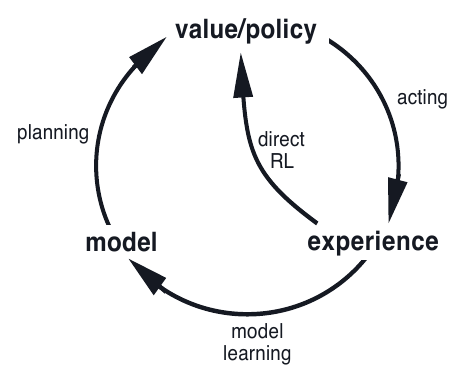
\includegraphics[width=0.45\textwidth]{Dyna_struct_1.png}}
    \subfigure[]{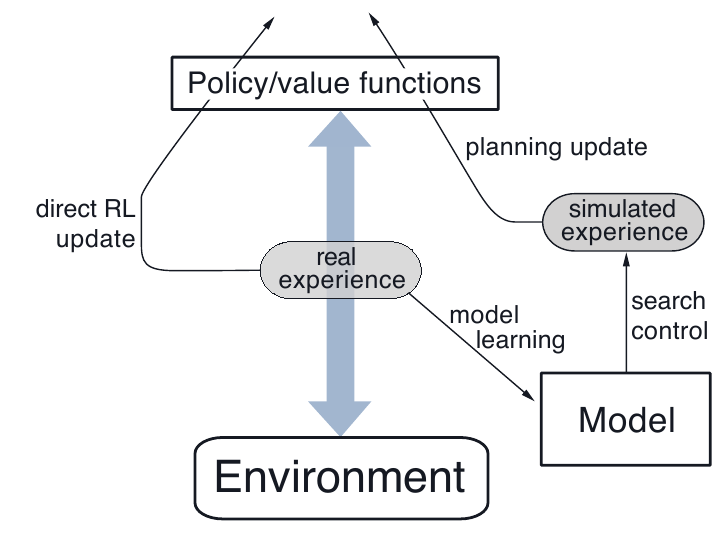
\includegraphics[width=0.45\textwidth]{Dyna_struct_2.png}}
    \caption{ (a) Dyna, balancing decision making and model learning (b) General Dyna Architecture }
    \label{fig:dyna}
\end{figure}

\begin{itemize}
\item real experience: (1) \textit{model-learning} (or indirect RL) to improve model (more accurately match the real environment); (2) \textit{direct RL} to improve value function and policy
\begin{itemize}
	\item indirect methods: maximize the use of limited experience (better policy with fewer environmental interactions)
	\item direct methods are more simpler and are not affected by biases incurred by the model
\end{itemize}
\item all planning, acting, model-learning, and direct RL occurring continually
\begin{itemize}
	\item planning here uses random-sample one-step tabular Q-\textbf{planning}
	\item direct RL here uses one-step tabular Q-\textbf{learning}
\end{itemize}
\item \textit{search control} to refer to the process that selects the starting states and actions for the simulated experiences generated by the model
\end{itemize}

\begin{figure}[!h]
  \centering
  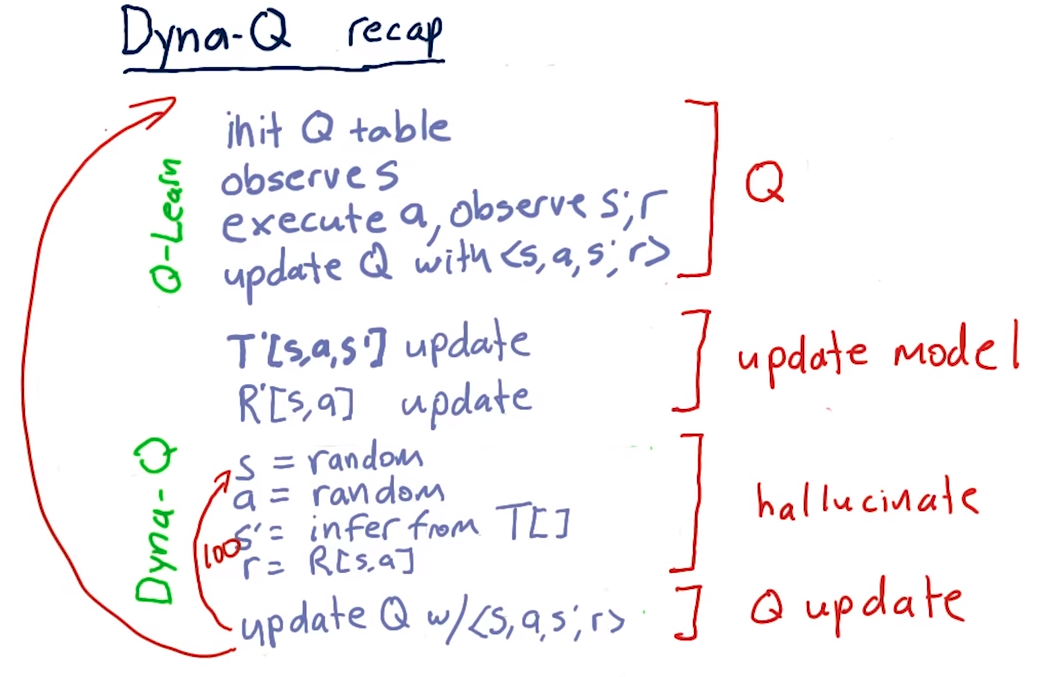
\includegraphics[width=0.6\linewidth]{dyna_3.png}
  \label{fig:dyna3}
\end{figure}

The Dyna Q uses both real world experience (which is expensive) and simulated (hallucinated) experience (which is cheap; more iterations are completed with simulated experience), thus accelerating training. The real experience is for learning, and simulated experience is for planning.

\begin{tcolorbox}[width=1.1\textwidth,title={Tabular Dyna-Q}]
Init $Q(s,a)$ and $Model(s,a)$ for all $s \in S$ and $a \in \A(s)$

Loop forever:

$\quad$(a) $S \leftarrow$ current (nonterminal) state

$\quad$(b) $A \leftarrow \epsilon$-greedy$(S,Q)$

$\quad$(c) Take action $A$; observe resultant reward, $R$, and state, $S'$

$\quad$(d) $Q(S,A)\leftarrow Q(S,A)+\alpha [R + \gamma max_a Q(S',a) - Q(S,A)]$

$\quad$(e) $Model(S,A) \leftarrow R,S'$ (assuming deterministic environment)

$\quad$(f) Loop repeat $n$ times:

$\quad\quad$ $S \leftarrow$ random previously observed state

$\quad\quad$ $A \leftarrow$ random action previously taken in $S$

$\quad\quad$ $R, S' \leftarrow Model(S,A)$

$\quad\quad$ $Q(S,A)\leftarrow Q(S,A)+\alpha [R+\gamma max_a Q(S',a) - Q(S,A)]$
\end{tcolorbox}

\subsection{When the Model Is Wrong}

The model learning in the Dyna-Q may be incorrect when encountering stochastic environment. The model may not be exploratory enough to find the new (optimal) path when environment changes, sticking to the old path. We slightly modified the reward transition in Dyna-Q+ with $r+\kappa\sqrt{\tau}$ for small $\kappa$, where $\tau$ is the time steps that the $(s,a)$ has not been tried (similar to how UCB incorporate time steps inside).

Read Blocking Task and Shortcut Task Examples in the book.

\subsection{Prioritized Sweeping}

Problem: search control select (s,a) uniform-randomly. Some (s,a) are not worth visiting

Solution: prioritized sweeping

! \textbf{Backward-focusing } of planning computations: in general, we want to work back not just from goal states but from any state whose value have changed.

As the frontier of useful updates propagates backward, it grows rapidly, producing many (s,a) that could be updated. But not all of them are equally useful. The value of some states have changed a lot, and the value of their predecessors are also likely to change a lot. It is then natural to prioritize them according to a measure of their urgency, and perform them in order of priority.

This is \textbf{prioritized sweeping}. A queue is maintained for every (s,a) whose value would change if updated, prioritized by the size of the change.

\begin{figure}[h!]
    \centering
    \subfigure[]{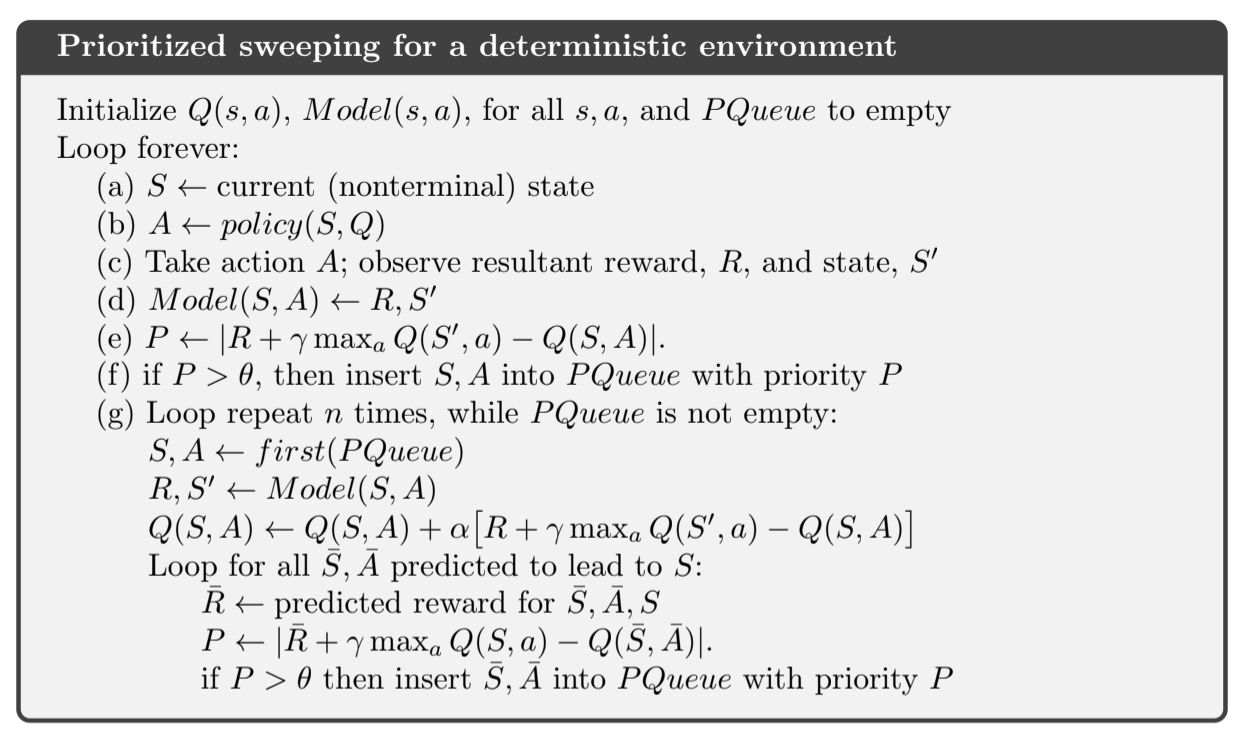
\includegraphics[width=0.8\textwidth]{prioritized_sweeping.png}}
    \caption{ Prioritized sweeping algorithm (deterministic environment) }
\end{figure}



\subsubsection{What about stochastic environment}

The model is maintained by keeping counts of the number of times each (s,a) has been experienced and what their next states were. We can update each (s,a) not with a sample update but with an \textbf{expected update}, taking into account the possibilities of the next states and their probability of occurring.

Using expected updates can waste a lot of computation on low-probability transitions. Often using samples help converge faster despite the added variance. Sample updates can be better because they break the overall backing-up computation into smaller pieces (individual transitions) which enables them to be more focused on the pieces that would have the greater impact.



We have focused on backward focusing, but this is only one strategy. Another could be to focus on states, according to how easy they can be reached from the states that are visited frequently under the current policy, which is \textbf{forward focusing}.

\subsection{Expected vs. Sample update}

We have considered many value-function updates. If we focus on one-step upates, they vary along 3 dimensions:
\begin{itemize}
\item Update state value or action values
\item Estimate the value of the optimal policy or any given policy
\item The updates are expected updates (consider all possible events) or sample updates (consider a sample of what might happen)
\end{itemize}
These 3 binary dimensions give rise to 8 cases, seven of which are specific algorithms.
Any of these one-step method can be used in planning methods. The Dyna-Q use $q_*$ sample update, but it can also use $q_*$ expected update or $q_\pi$ update.

\begin{figure}[h!]
    \centering
    \subfigure[]{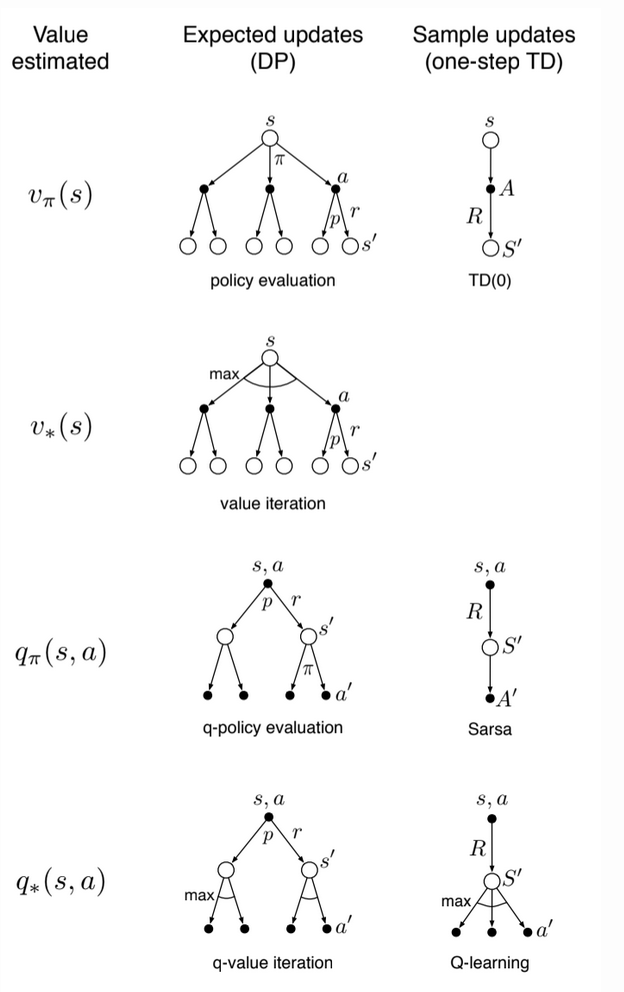
\includegraphics[width=0.8\textwidth]{dimensions.png}}
    \caption{ Backup diagrams for one-step updates }
\end{figure}

When we don’t have the environment model, we can’t do an expected model so we use a sample. But are expected update better than sample updates when available?

(1) they yield a better estimate because they are uncorrupted by sampling error; (2) but they require more computation

\subsubsection{computational requirements}

For $q_*$ approximation in this setup
\begin{itemize}
\item discrete states and actions
\item table-lookup representation of the approximate value function Q
\item a model in the form of estimated dynamics $\hat{p}(s',r|s,a)$
\end{itemize}
The expected update is:
$$ Q(s, a) \gets \sum_{s', r} \hat{p}(s', r|s, a) \big[r + \gamma \underset{a'}{\mathrm{max}} Q(s', a')\big] $$
The sample update is (Q-learning like):
$$ Q(s, a) \gets Q(s, a) + \alpha \big[ R + \gamma \underset{a'}{\mathrm{max}} Q(S', a') - Q(s, a)\big] $$

expected update vs.sample update: difference depends on stochasticity of the environment.

Many possible next states = many computation for the expected update.

For a particular set $(s,a)$, let $b$ be the branching factor (the number of possible next states). Then an expected update of this pair requires roughly $b$ times as much computation as a sample update.

\begin{figure}[h!]
    \centering
    \subfigure[]{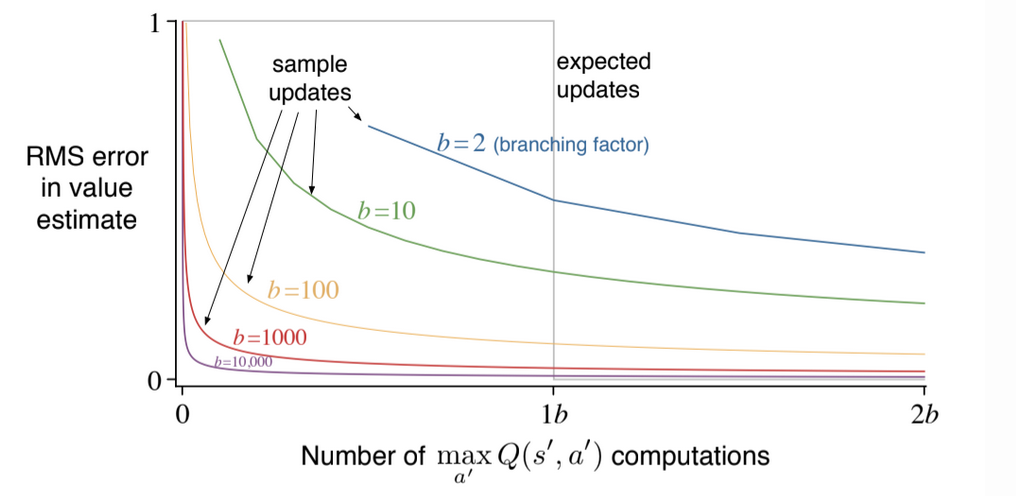
\includegraphics[width=0.8\textwidth]{computation.png}}
    \caption{ Comparison of the efficiency of expected and sample updates }
\end{figure}

conclusion: sample updates are better to expected updates on problems with a large branching factor and too many states


\subsection{Trajectory Sampling}

2 ways of distributing updates:
\begin{itemize}
\item \textbf{exhaustive sweep} (classical approach from DP): perform sweeps through the entire state space, updating each state once per sweep
\item sample from the state space according to some distribution
\begin{itemize}
	\item uniform sample: Dyna-Q
	\item on-policy distribution (interact with the model following the current policy). Sample state transitions and rewards are given by the model, and sample actions are given by the current policy. We simulate explicit individual trajectories and perform update at the state encountered along the way -> \textbf{trajectory sampling}
\end{itemize}
\end{itemize}

Is the on-policy distribution a good one?
\begin{itemize}
\item it causes vast, uninteresting parts of the space to be ignored
\item could be bad because we update the same parts over and over
\end{itemize}

conclusion:
\begin{itemize}
\item in the long run (and/or small problems), exhaustive sampling
\begin{itemize}
	\item Focusing on the on-policy distribution may hurt in the long run because the commonly occurring states all already have their correct value. Sampling them is useless.
\end{itemize}
\item large problems, on-policy sampling/distribution
\end{itemize}

\subsubsection{Real-Time Dynamic Programming (RTDP)}

RTDP is an on-policy trajectory-sampling version of the value-iteration algorithm of DP. It is closely related to full-sweep policy iteration so we illustrate some advantages that on-policy trajectory sampling can have.

RTDP updates the values of states visited in actual or simulated trajectories by means of expected tabular value-iteration updates.

RTDP is an example of an asynchronous DP algorithm. Asynchronous algorithms do not do full sweeps, they update state values in any order, using whatever value of other states happen to be available. In RTDP, th update order is dictated by the order states are visited in real or simulated trajectories.

\subsubsection{Evaluation}

\begin{figure}[h!]
    \centering
    \subfigure[]{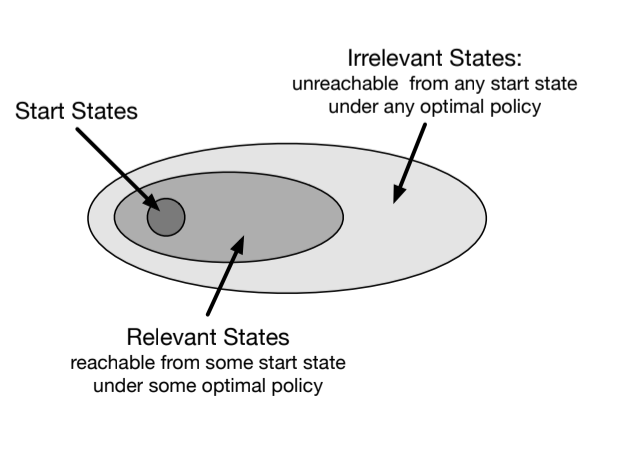
\includegraphics[width=0.8\textwidth]{rtdp.png}}
    \caption{ Classification of states }
\end{figure}

\begin{itemize}
\item trajectories start from a designated set of start states
\item we have a prediction problem for a given policy
\item on-policy trajectory sampling allows to focus on useful states
\end{itemize}

\subsubsection{Improvement}

For Control, the goal is to find an optimal policy instead of evaluating a given policy, there might be states that cannot be reached by any of the optimal policies from any of the start states, so there is no need to specify optimal actions for those irrelevant states. We in fact only need an optimal partial policy.

Finding such an optimal partial policy can require visiting all state-action pairs, even those turning out to be irrelevant in the end. It is generally not possible to stop updating any state if convergence to an optimal policy is important.

For certain types of problems under certain conditions, RTDP is guaranteed to fin a policy that is is optimal on the relevant states without visiting every state infinitely often, or even without visiting some states at all.

The task must be an undiscounted episodic task for MDP with absorbing goal state that generate zero reward.

At every step or a real or simulated trajectory, RTDP selects a greedy action and applies the expected value-iteration update operation to the current state. It can also update other states, like those visited in a limited-horizon look-ahead search from the current state.

More conditions for guarantee of optimal convergence:

\begin{itemize}
\item the initial value of every goal state is 0
\item there exists at least one policy that guarantees a goal state will be reached from any start state
\item all rewards from transitions from non-goal states are strictly negative
\item the initial values are $\geq$ to optimal values

\end{itemize}

Proof: Barto, Bradtke and Singh 1995

Tasks having these properties are examples of stochastic optimal path problems, which are usually stated in term of cost minimization instead of reward maximization, but we can just maximize the negative returns.

\subsection{Planning at Decision Time}
Two ways to plan:
\begin{itemize}
\item background planning (Dyna, DP)
\item decision-time planning: begin and complete planning \textit{after} encountering each state $S_t$, to produce a single action $A_t$.
\end{itemize}

\subsection{Heuristic search}

The classical state-space plannng methods are decision-time planning methods collectively known as heuristic search. In heuristic search, for each state encountered, a large tree of possible continuations is considered. The approximate value function is applied to the leaf nodes and then backed up toward the current state at the root, then the best is chosen as the current action, and all other backed-up values are discarded.

\subsection{Rollout algorithms}

skip

\subsection{MCTS}

skip


\subsection{Learning Objectives (UA RL MOOC)}


Lesson 1: What is a model? 

1. Describe what a model is and how they can be used

\begin{itemize}
\item Model are used to store knowledge about the transition and reward dynamics
\item Given $S,A$ into model, model outputs $R, S'$
\item A model allows for planning
\item Planning refers to the process of using a model to improve a policy (use model to simulate experience, update value functions with the simulated experience, then improve policy with the updated value functions)
\end{itemize}

2. Classify models as distribution models or sample models 

\begin{itemize}
\item Sample models procedurally generate samples, without explicitly storing the probability of each outcome (e.g. flip coin twice: HT)
\item Distribution models contain a list of all outcomes and their probabilities (e.g. flip coin twice HT(1/4),HH(1/4),TT(1/4),TH(1/4))
\end{itemize}

3. Identify when to use a distribution model or sample model 

Sample model can be computationally inexpensive. Distribution model contains more info, but it's hard to specify and can become large.

4. Describe the advantages and disadvantages of sample models and distribution models 

Sample models require less memory

Distribution models can be used to compute the exact expected outcome (note sample models have to averaging many samples to get an approximate). Can be used to access risk.

5. Explain why sample models can be represented more compactly than distribution models

Consider rolling dice sample. The more dice there are, the larger the state space.

Lesson 2: Planning 

6. Explain how planning is used to improve policies 

Planning uses simulated experience from model to improve policies.

7. Describe random-sample one-step tabular Q-planning 

(1) sample from model; (2) Q-learning update; (3) Greedy policy improvement

Lesson 3: Dyna as a formalism for planning 

8. Recognize that direct RL updates use experience from the environment to improve a policy or value function 

Direct RL, like Q-learning, directly learn from real world experience (environment)

9. Recognize that planning updates use experience from a model to improve a policy or value function 

Indirect RL, like Q-planning, learn from simulated experience (generated by model) to improve value function and policy.

10. Describe how both direct RL and planning updates can be combined through the Dyna architecture

see \ref{fig:dyna} we do direct RL with real experience to improve policy or value functions; and we learn a model use real experience, then we sample (state, action) from the model which we use to get simulating experience, and we do planning update based on simulated experience to update policy or value functions

11. Describe the Tabular Dyna-Q algorithm 

see Chap 8.2

12. Identify the direct-RL and planning updates in Tabular 

direct RL update is the step (d), planning update is step (f)

13. Identify the model learning and search control components of Tabular Dyna-Q 

10-13 see chap 8.2

14. Describe how learning from both direct and simulated experience impacts performance 

It accelerate learning and it also very sample efficient.

15. Describe how simulated experience can be useful when the model is accurate 

It can provide more samples for training, thus it's improve sample efficiency.

Lesson 4: Dealing with inaccurate models 

16. Identify ways in which models can be inaccurate 

Models are inaccurate when transitions they store are different from transitions that happen in the environment (like haven't explore enough or the environment is nonstationary / changing).


17. Explain the effects of planning with an inaccurate model 

At first, the model is incomplete. As the agent interacts with the environment, the model stores more and more transitions. Then, the agent can perform updates by simulating transitions it's seen before. That means that as long as the agent has seen some transitions, it can plan with the model.

If the agent plan to with inaccurate model, then the value function or policy that the agent updates might change in the wrong direction. Planning with inaccurate model can make the policy worse w.r.t the environment.

18. Describe how Dyna can plan successfully with a partially inaccurate model 

In the step (f), the model only knows the next state and reward from $(s,a)$ it has already visited; therefore, Dyna-Q can only do planning updates from previously visited $(s,a)$ pairs. Dyna-Q only plans the transition it has already seen. So in the first few timesteps of learning, Dyna-Q might do quite a few planning updates with the same transition. However, as Dyna-Q visits more $(s,a)$ in the environment, its planning updates become more evenly distributed throughout the state action space.

19. Explain how model inaccuracies produce another exploration-exploitation trade-off 

Explore to make sure its model is accurate, exploit the model to compute the optimal policy, assuming that the model is correct.

20. Describe how Dyna-Q+ proposes a way to address this trade-off

We add a bonus rewards for exploration, new reward = $r + \kappa\sqrt{\tau}$, where $\kappa$ is small constant and $\tau$ is timesteps since transition was last tried.

21. (new research area?) We can have a separate thread (multi-threading) for planning specifically.

22. UCB method is similar to the bonus reward of Dyna-Q+: the difference is that they use differently (UCB can't work with nonstationary problems)

23. (new research area?) We start an easy and safe environment for the agent then we gradually make the environment more realistic/dangerous to the agent.

\end{document}